\chapter{Esperimenti di simulazione}\label{chp:esperimenti-simulazione}
In accordo agli obiettivi dello studio, per la progettazione degli esperimenti di simulazione, è stata considerata unicamente l'analisi dello stato transiente del sistema. Infatti, perderebbe di significato considerare lo stato stazionario per determinare il numero minimo di serventi necessari affinché vengano soddisfatti i QoS descritti nel capitolo \ref{chp:obiettivi}. Questo perché in una giornata lavorativa, assunta pari ad otto ore, il sistema non riesce a raggiungere lo stato stazionario prima che si verifichi la condizione di scarico (\textit{"close the door"}) ed inoltre rimane forte l'influenza delle condizioni iniziali.

\begin{figure}[ht]
\centering
\begin{subfigure}[b]{0.475\textwidth}
\centering
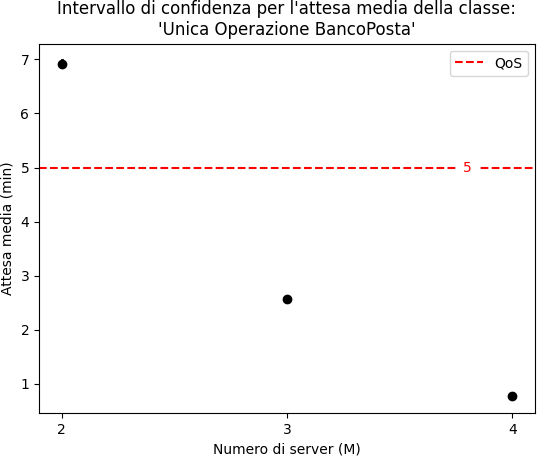
\includegraphics[width=\textwidth]{plots/d0-trans}
\caption{Tempo medio d'attesa per ticket di tipo 0}    
\label{fig:esperimenti-simulazione-a}
\end{subfigure}
\hfill    
\begin{subfigure}[b]{0.475\textwidth}  
\centering 
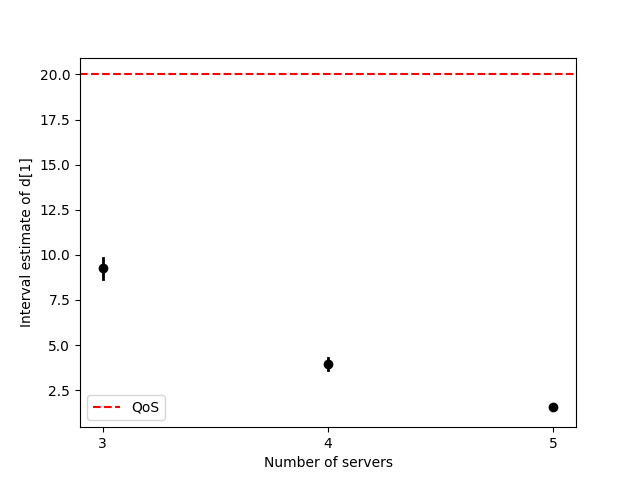
\includegraphics[width=\textwidth]{plots/d1-trans}
\caption{Tempo medio d'attesa per ticket di tipo 1}    
\label{fig:esperimenti-simulazione-b}
\end{subfigure}


\vskip\baselineskip

\begin{subfigure}[b]{0.475\textwidth}   
\centering 
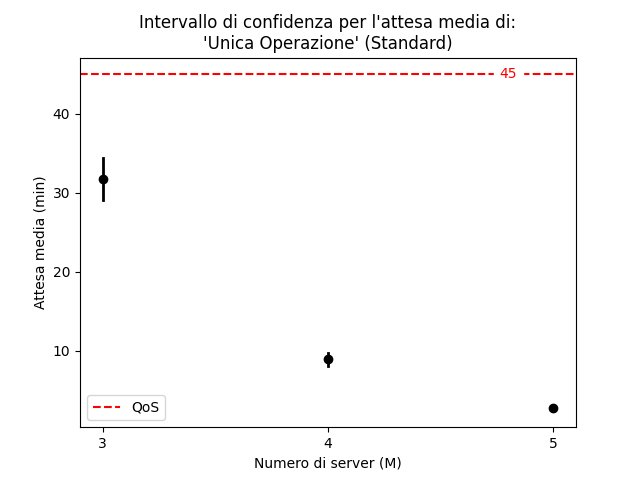
\includegraphics[width=\textwidth]{plots/d2-trans}
\caption{Tempo medio d'attesa per ticket di tipo 2}    
\label{fig:esperimenti-simulazione-c}
\end{subfigure}
\hfill
\begin{subfigure}[b]{0.475\textwidth}   
\centering 
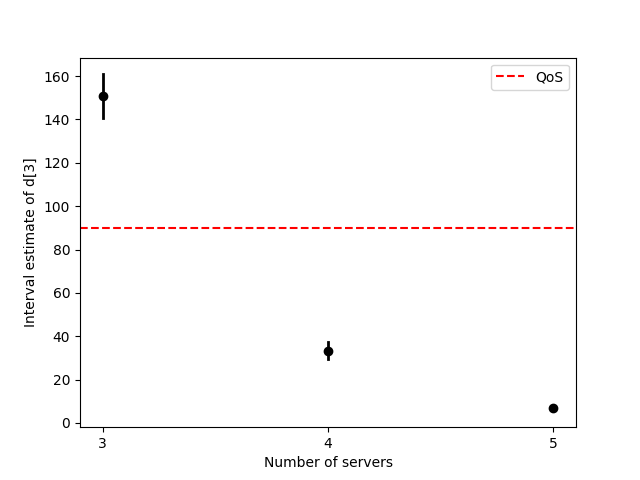
\includegraphics[width=\textwidth]{plots/d3-trans}
\caption{Tempo medio d'attesa per ticket di tipo 3}    
\label{fig:esperimenti-simulazione-d}
\end{subfigure}

\vskip\baselineskip

\begin{subfigure}[b]{0.475\textwidth}   
\centering 
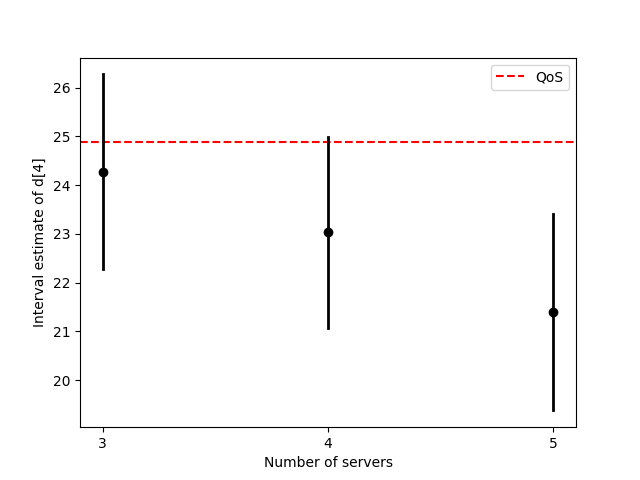
\includegraphics[width=\textwidth]{plots/d4-trans}
\caption{Tempo medio d'attesa per ticket di tipo 4}    
\label{fig:esperimenti-simulazione-e}
\end{subfigure}
\hfill
\begin{subfigure}[b]{0.475\textwidth}   
\centering 
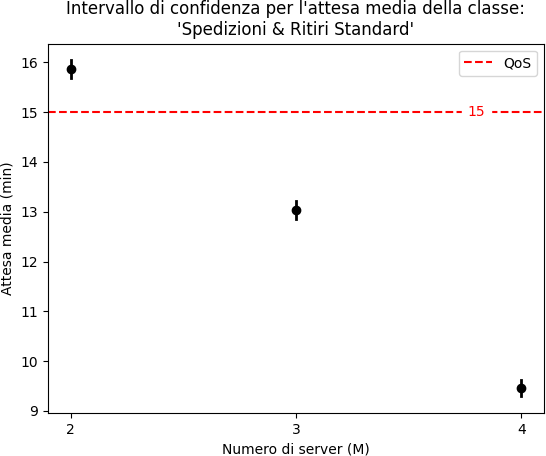
\includegraphics[width=\textwidth]{plots/d5-trans}
\caption{Tempo medio d'attesa per ticket di tipo 5}    
\label{fig:esperimenti-simulazione-f}
\end{subfigure}
\caption{Tempi medi d'attesa al variare di $M$ (id dei ticket in tabella \ref{table:modello-specifiche-1})}
\label{fig:verifica-1}
\end{figure}


